\newpage
\flushleft
\section*{Appendix B - 2D Open Flow Results} 
\addcontentsline{toc}{section}{Appendix B - 2D Open Flow Results}

\begin{figure}
    \centering
    \includegraphics[height=6.5cm]{Figures/2D_OF/2D_OF_MESH.png}
    \caption{General hybrid 2D open flow mesh consist of triangular and quadrilateral (inflation layer) mesh.}
    \label{fig:2D_OF_MESH}
\end{figure}

%%%%%%%%%%%%%%%%%%%%%%%%%%%%%
%%%   OPEN FLOW CONTOURs  %%%
%%%%%%%%%%%%%%%%%%%%%%%%%%%%%

\begin{figure}
    \noindent\makebox[\textwidth]{
    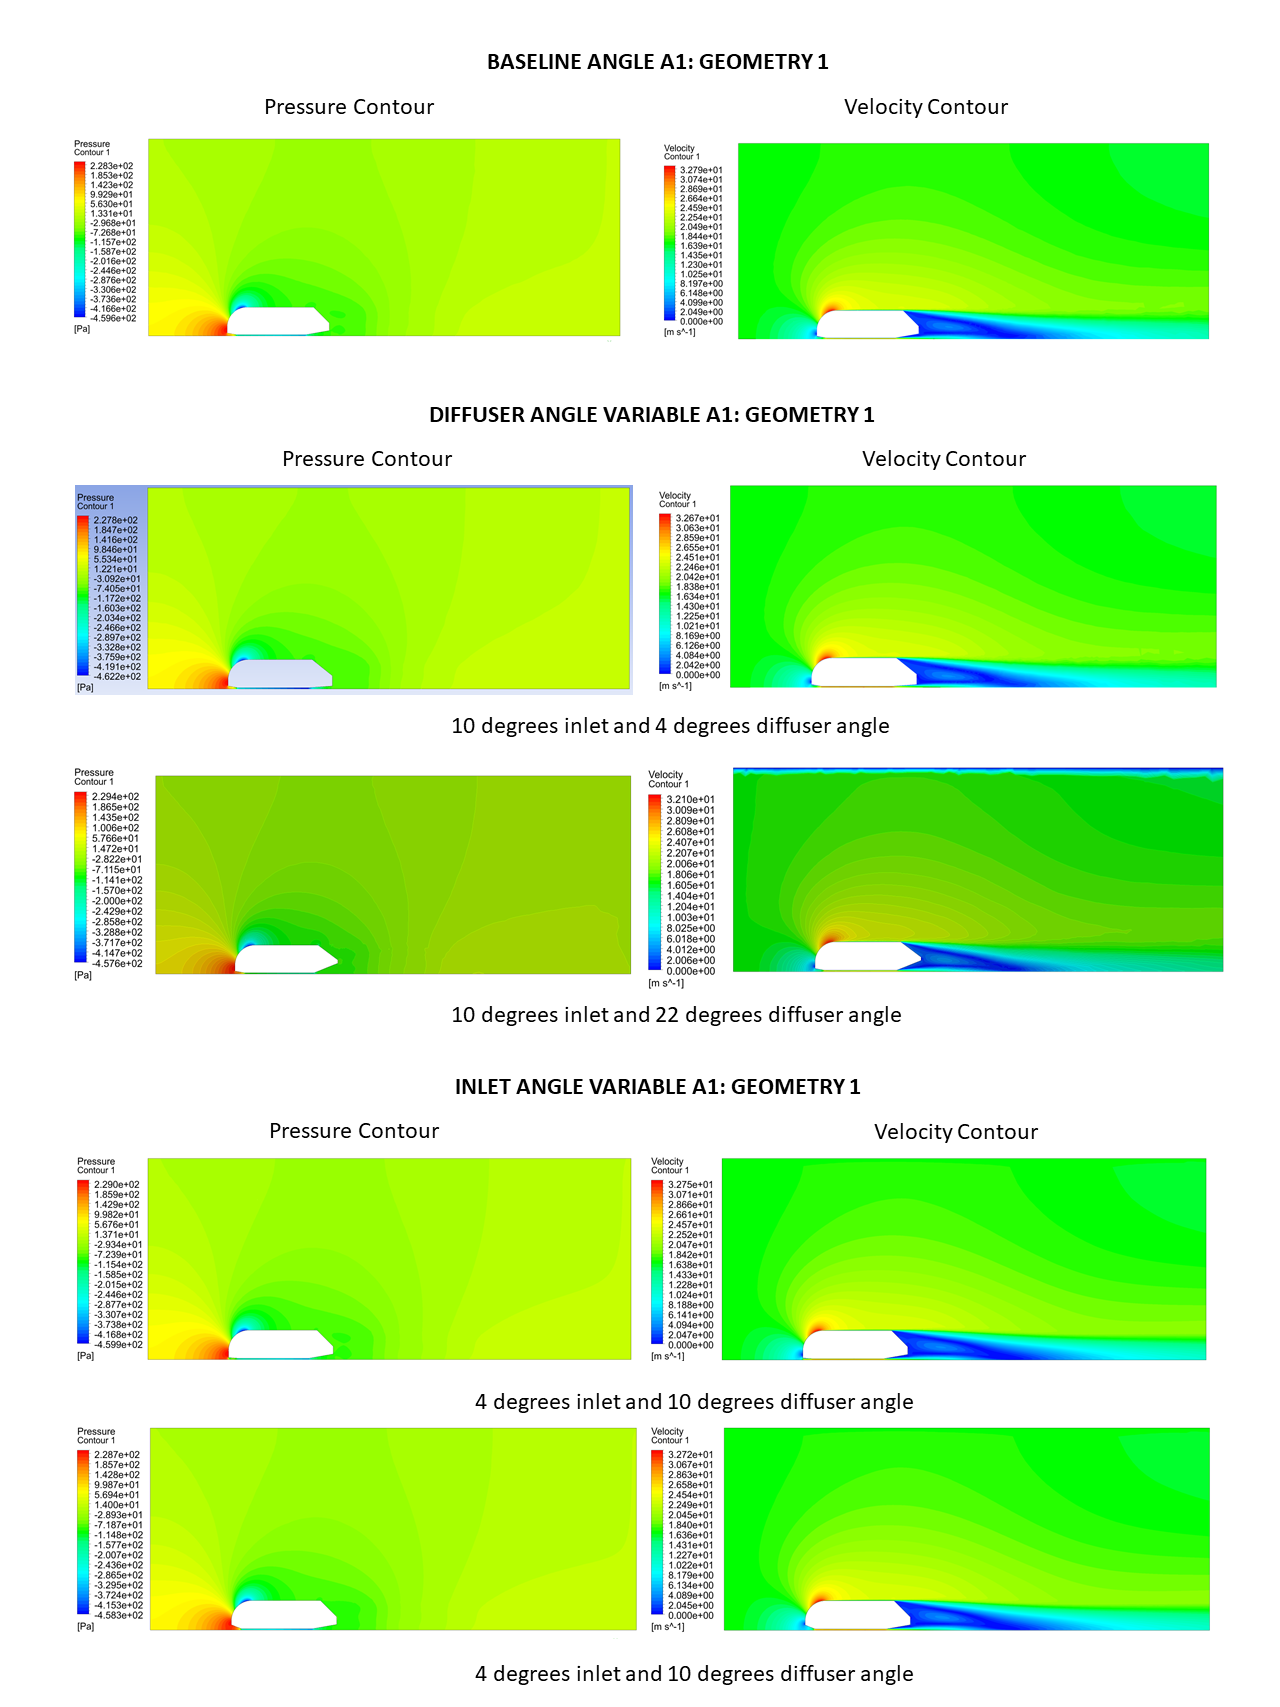
\includegraphics[width=1.1\textwidth]{Figures/2D_OF/A1_CONTOUR_ALL.PNG}}
    \caption{Pressure and velocity contour of A1: Geometry 1 in various angle variables.}
    \label{fig:2D_OF_A1_CONTOUR}
\end{figure}

\begin{figure}
    \noindent\makebox[\textwidth]{
    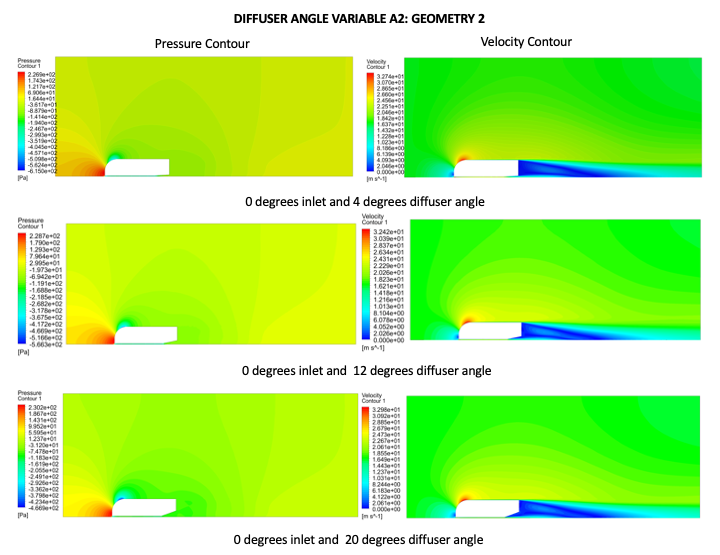
\includegraphics[width=1.1\textwidth]{Figures/2D_OF/A2_CONTOUR_ALL.png}}
    \caption{Pressure and velocity contour of A2: Geometry 2 in various diffuser angle.}
    \label{fig:2D_OF_A2_CONTOUR}
\end{figure}


\begin{figure}
    \noindent\makebox[\textwidth]{
    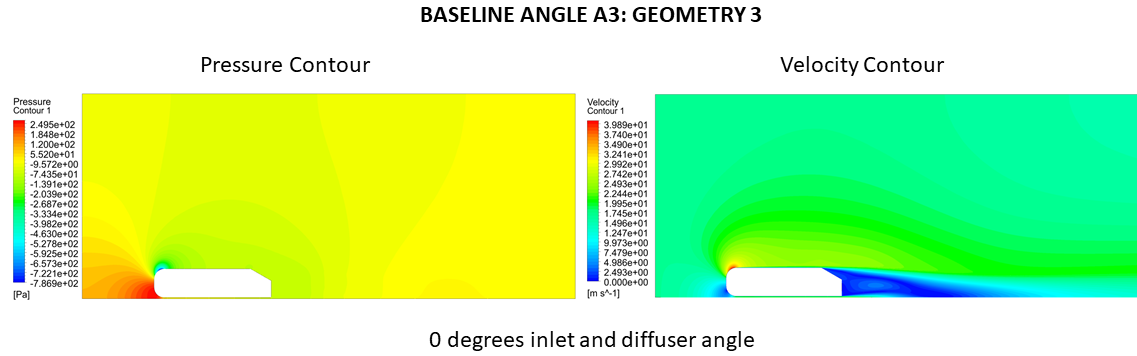
\includegraphics[width=1.1\textwidth]{Figures/2D_OF/A3_CONTOUR_ALL_1.PNG}}  
    \label{fig:2D_OF_A3_Contour1}
\end{figure}

\begin{figure}
    \noindent\makebox[\textwidth]{
    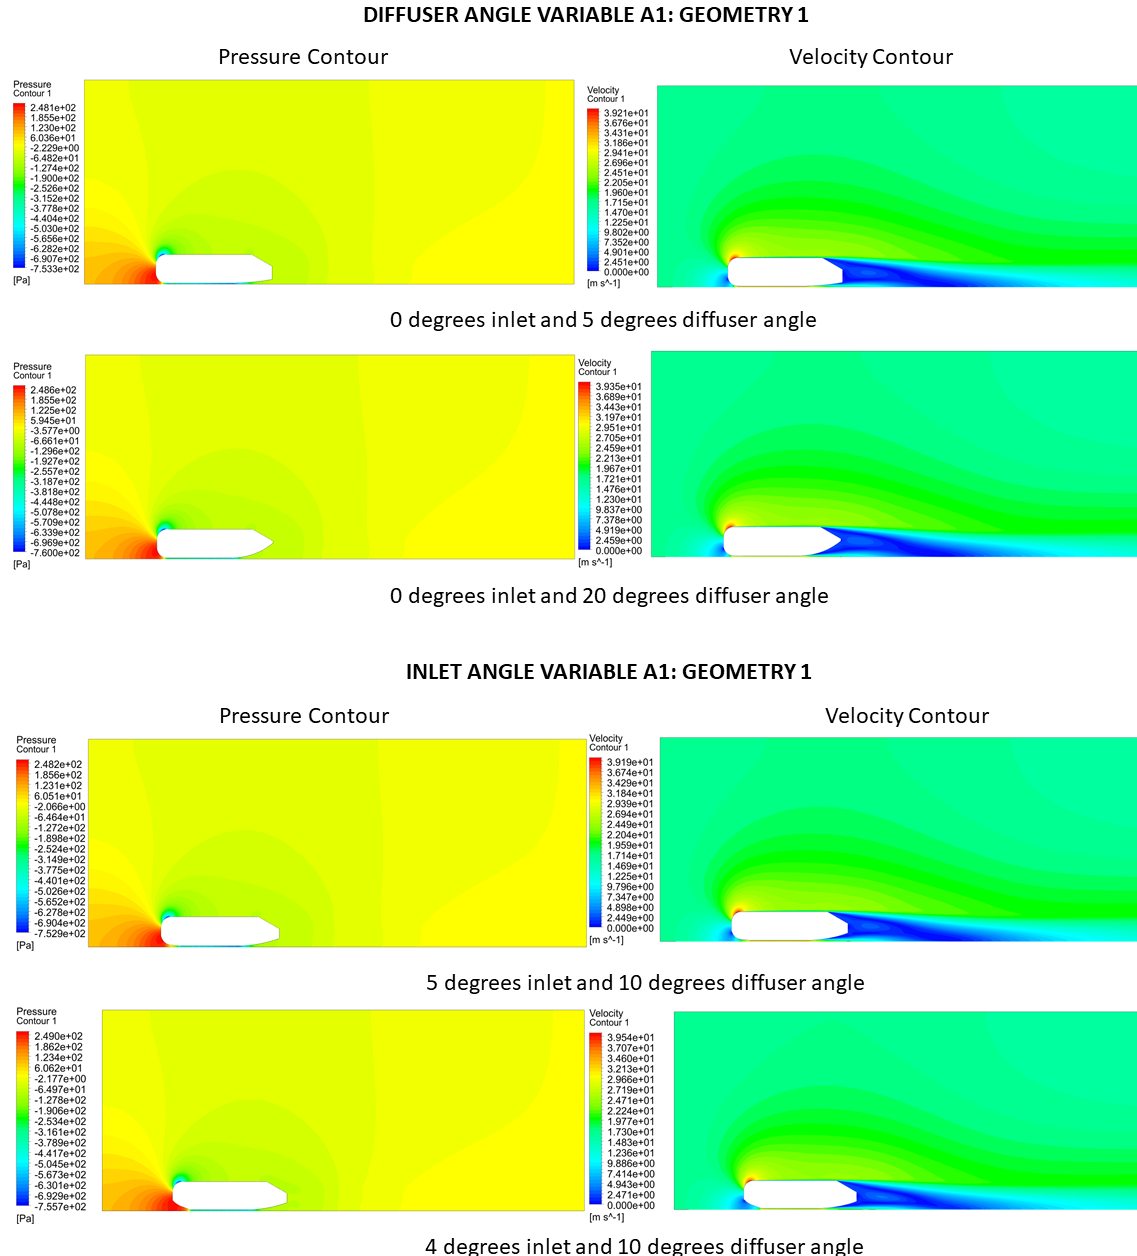
\includegraphics[width=1.1\textwidth]{Figures/2D_OF/A3_CONTOUR_ALL_2.PNG}}
    \caption{Pressure and velocity contour of A3: Geometry 3 in various angle variables.}
    \label{fig:2D_OF_A3_Contour2}
\end{figure}

%%%%%%%%%%%%%%%%%%%%%%%%%%%%%
%%% OPEN FLOW PLOT RESULT %%%
%%%%%%%%%%%%%%%%%%%%%%%%%%%%%

\begin{figure}
    \centering
    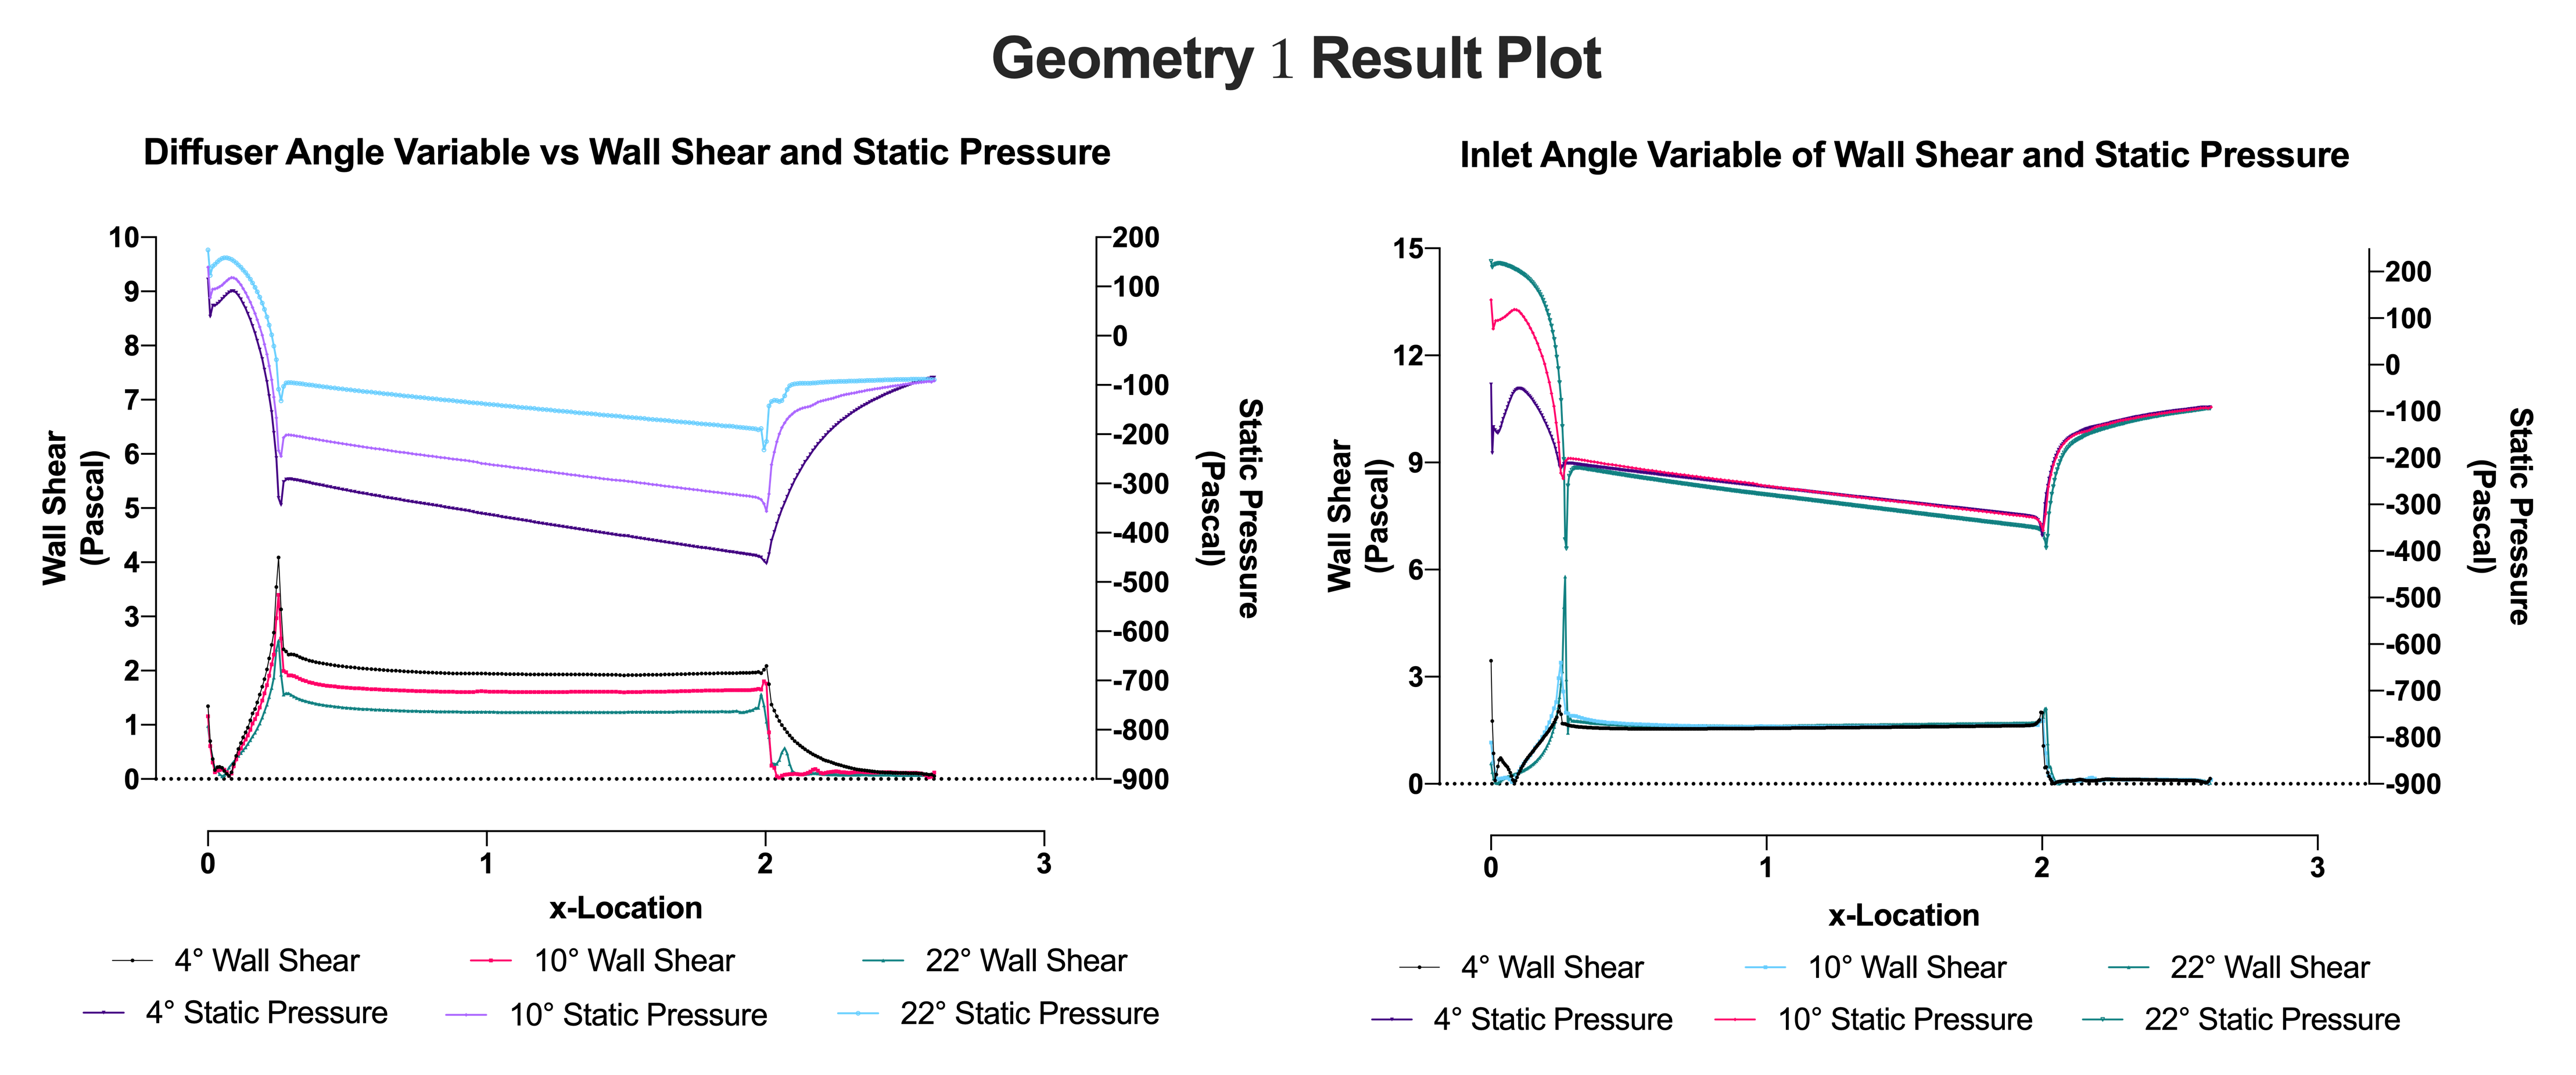
\includegraphics[scale=0.8]{Figures/2D_OF/2D_OF_A1_PRESS_WShear_PLOT.png}
    \caption{Diffuser (left) and Inlet (right) angle variable vs wall shear (bottom) and static pressure (top) of the undertray plot for geometry 1.}
    \label{fig:2D_OF_A1_PLOT}
\end{figure}

\begin{figure}
    \centering
    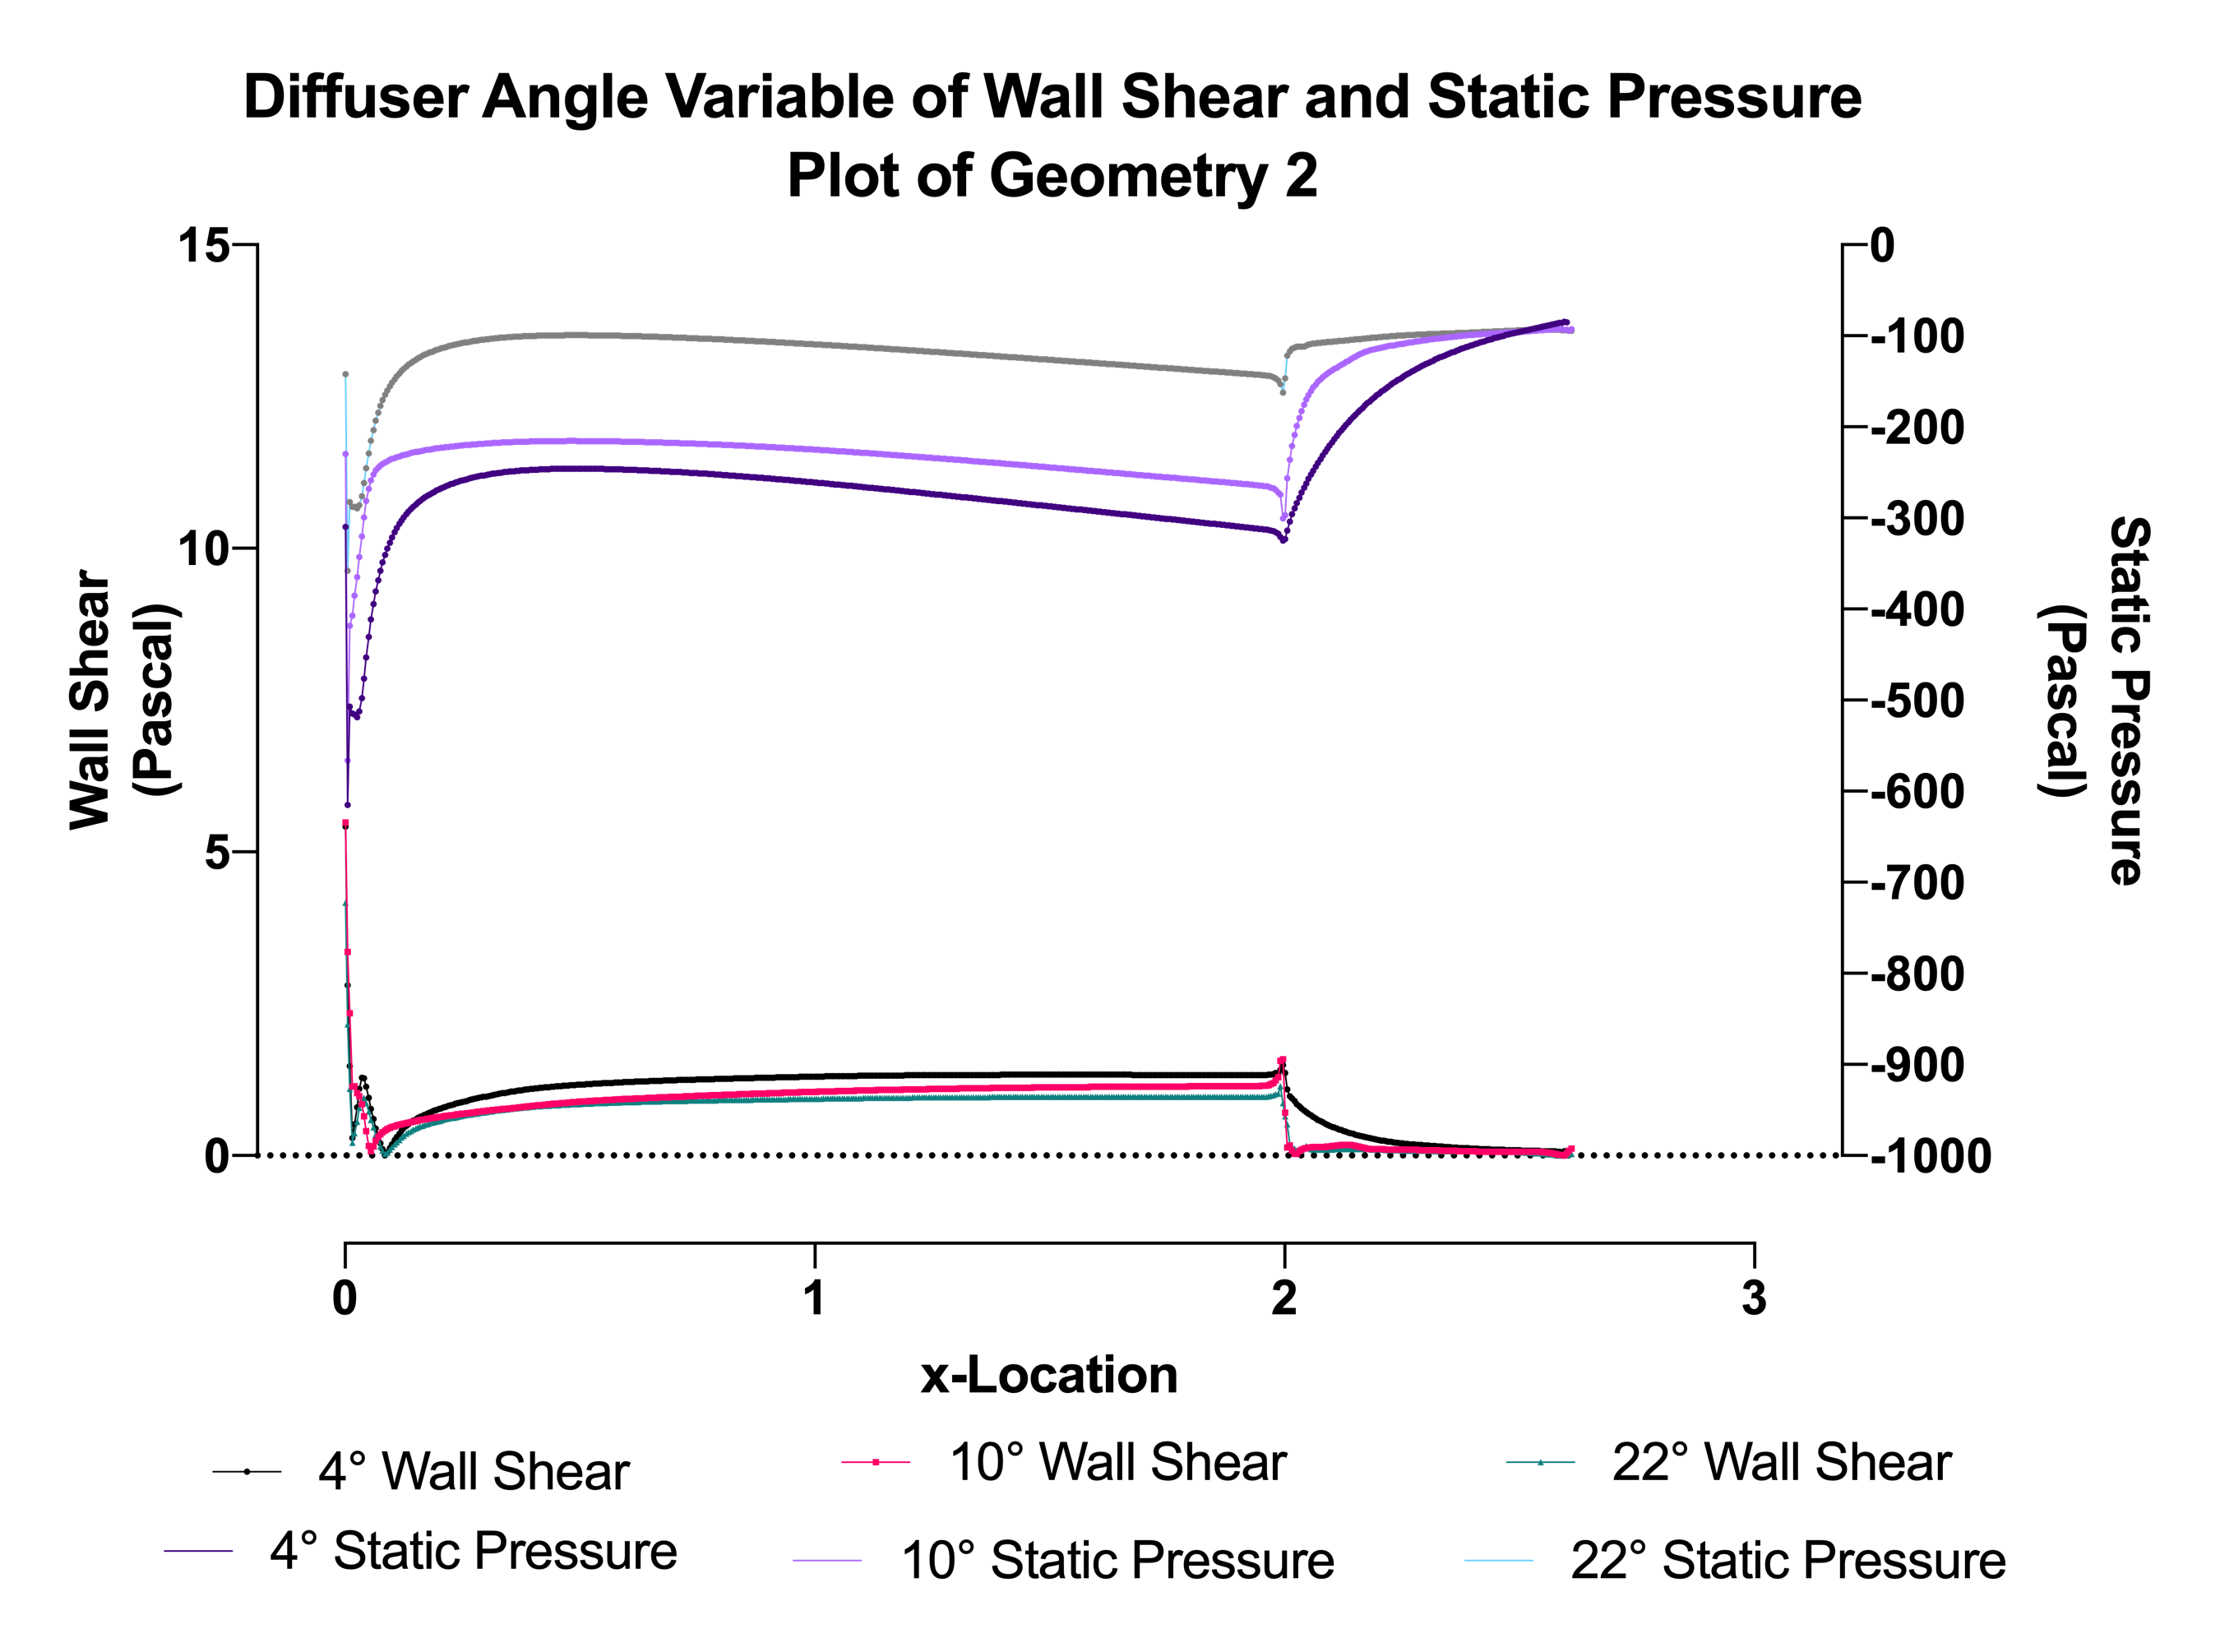
\includegraphics[scale=0.82]{Figures/2D_OF/2D_OF_A2_PRESS_WShear_PLOT.png}
    \caption{Diffuser angle variable vs wall shear (bottom) and static pressure (top) of the undertray plot for geometry 2.}
    \label{fig:2D_OF_A2_PLOT}
\end{figure}

\begin{figure}
    \centering
    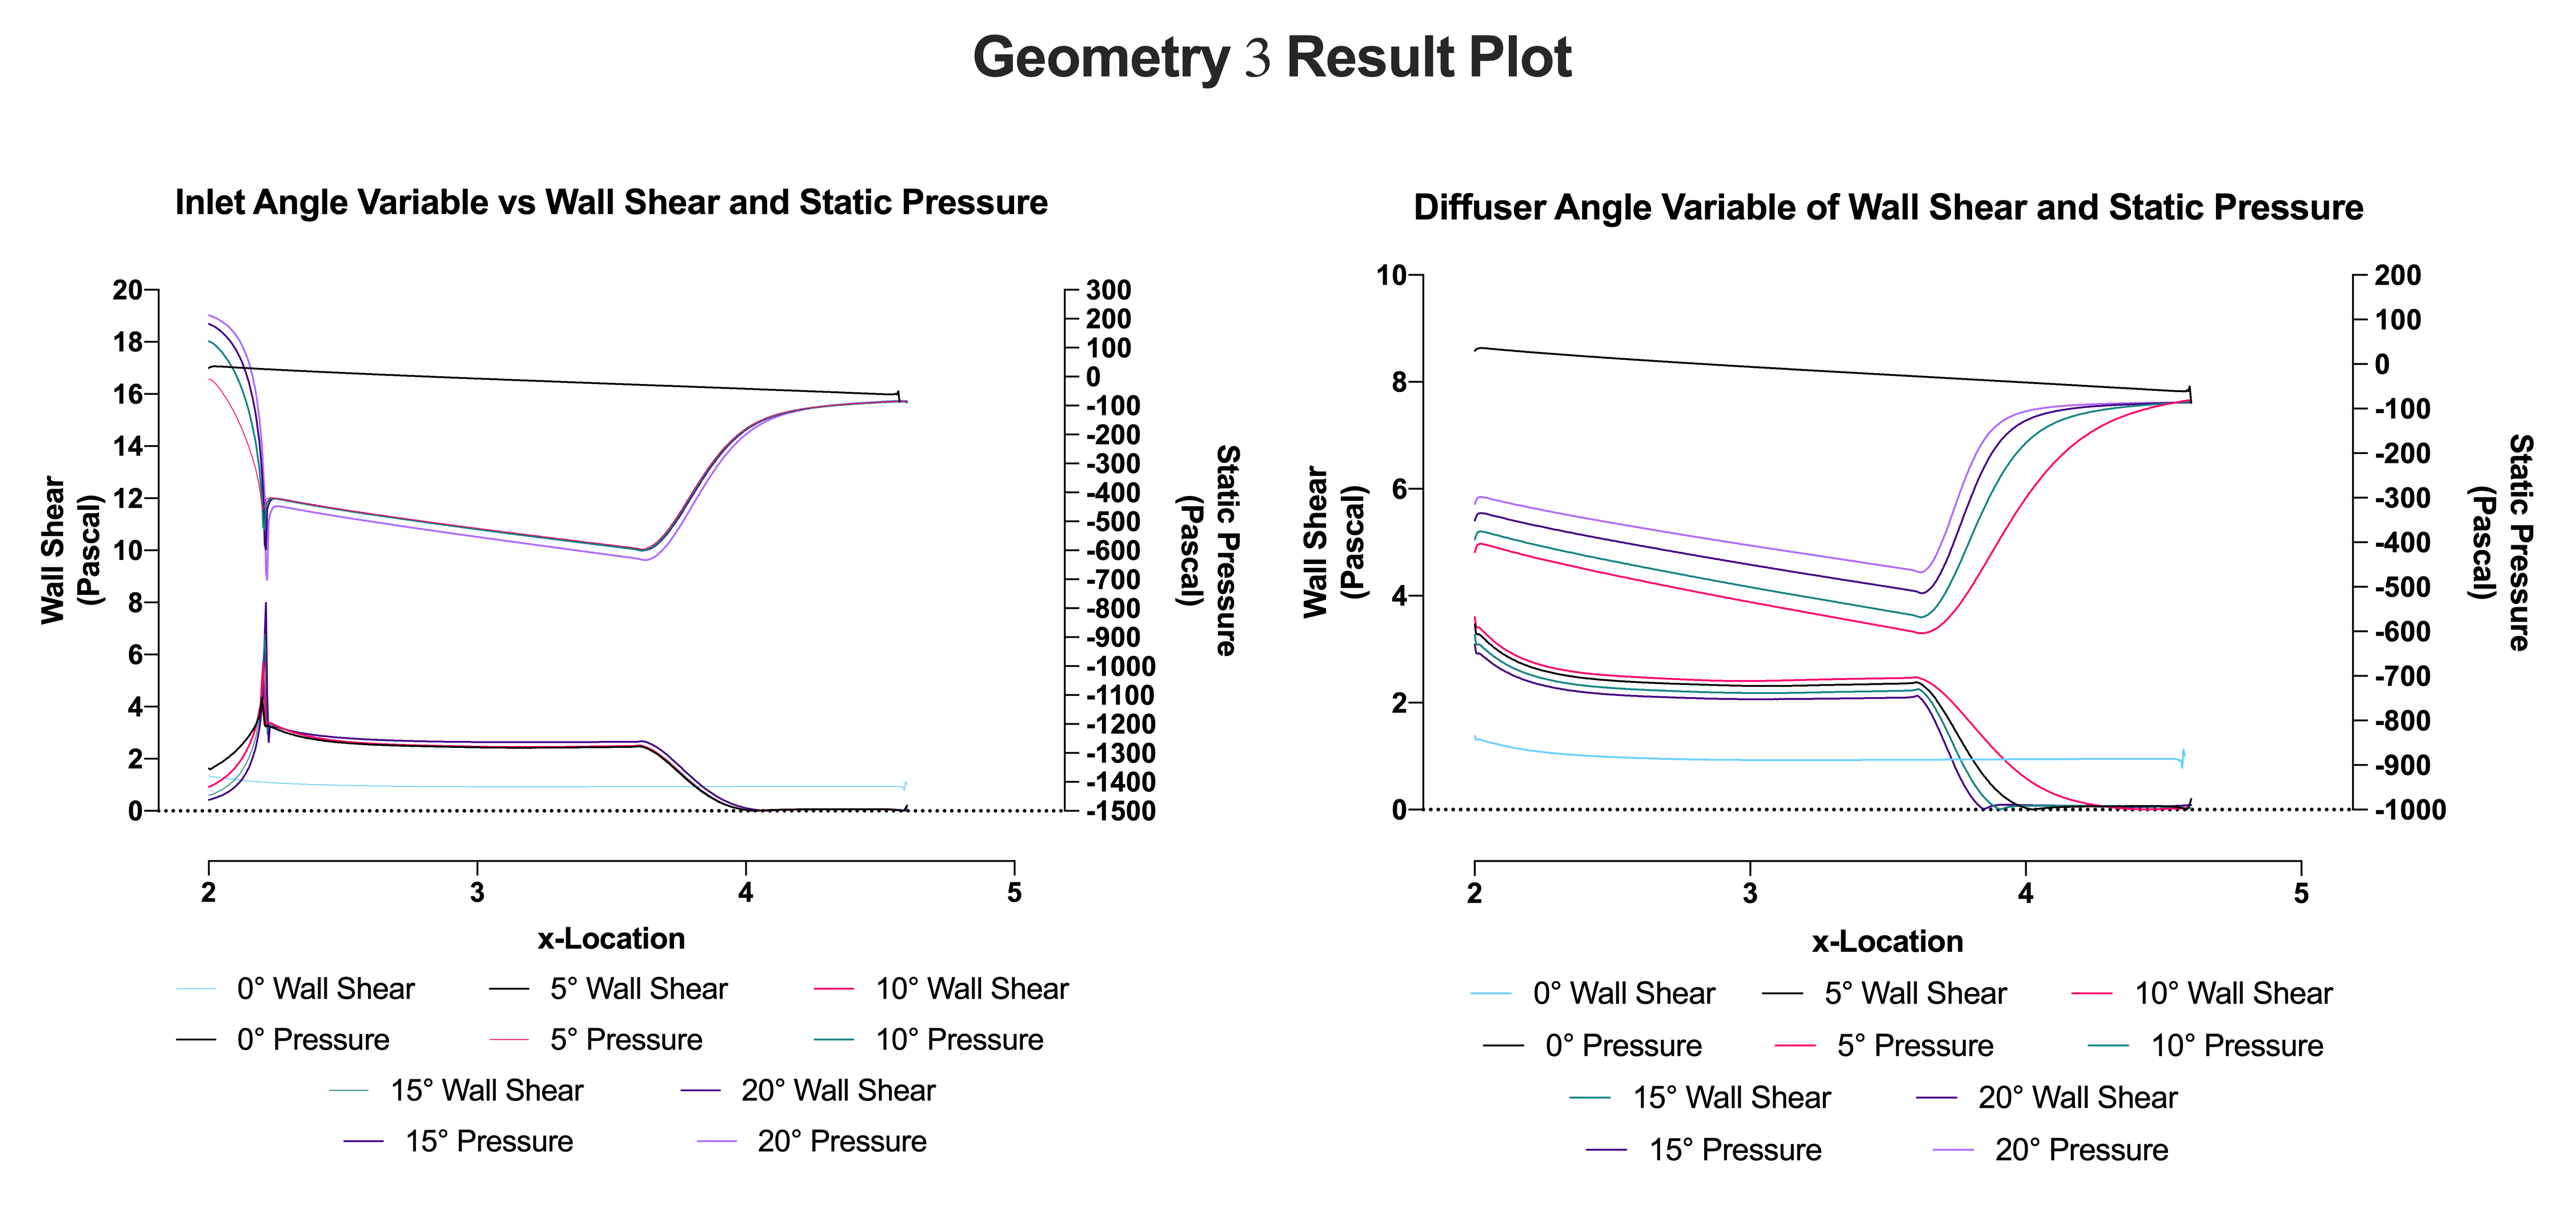
\includegraphics[scale=0.82]{Figures/2D_OF/2D_OF_A3_PRESS_WShear_PLOT.png}
    \caption{Inlet (left) and diffuser (right) angle variable vs wall shear (bottom) and static pressure (top) of the undertray plot for geometry 3.}
    \label{fig:2D_OF_A3_PLOT}
\end{figure}


